\section{Reinforcement Learning Interface}\label{sec:learning}

This section will present the concepts of the interface and discuss design decisions.
The interface should reflect experiments executed in our wrong and therefor only present information to the agent that realistic acquirable in our world, this is to intentionally limit what of the observable state is directly exposed the agent.

\begin{figure}
\centering
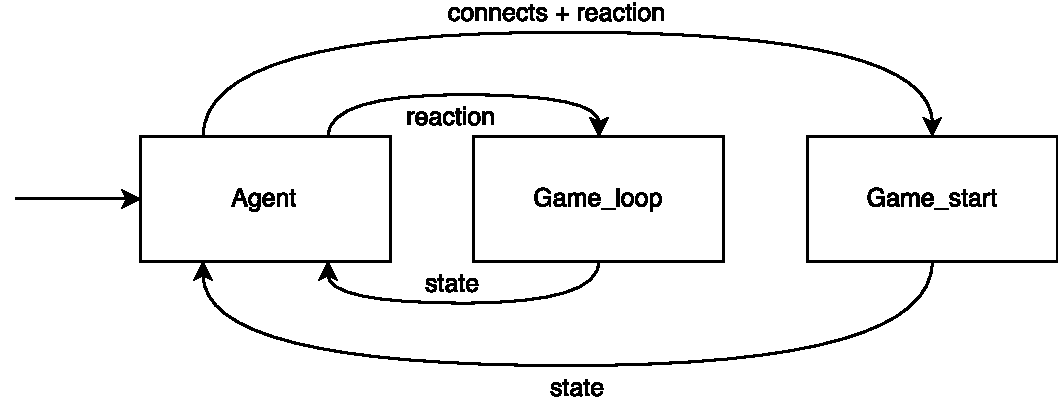
\includegraphics[width=.6\linewidth]{figures/neodroid_agent_game.pdf}
\caption{loop}
\label{fig:loop}
\end{figure}

Fig.~\ref{fig:loop} show the agent-environment loop.

\begin{figure}
\centering
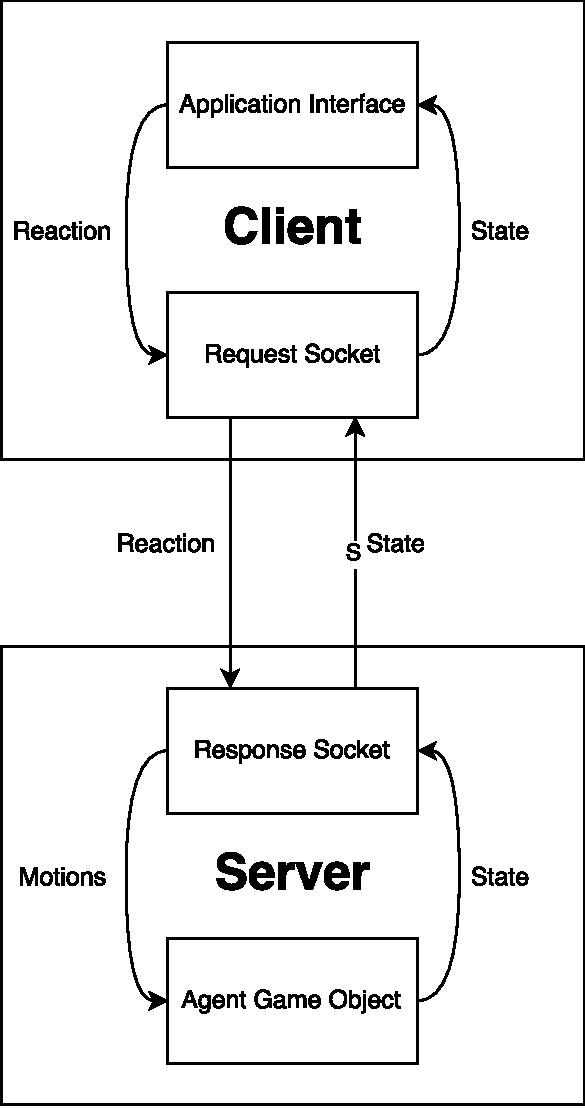
\includegraphics[width=.3\linewidth]{figures/networking.pdf}
\caption{networking}
\label{fig:networking}
\end{figure}

Fig.~\ref{fig:networking} show the agent-environment networking.


\subsection{Models}

\begin{figure}
\centering
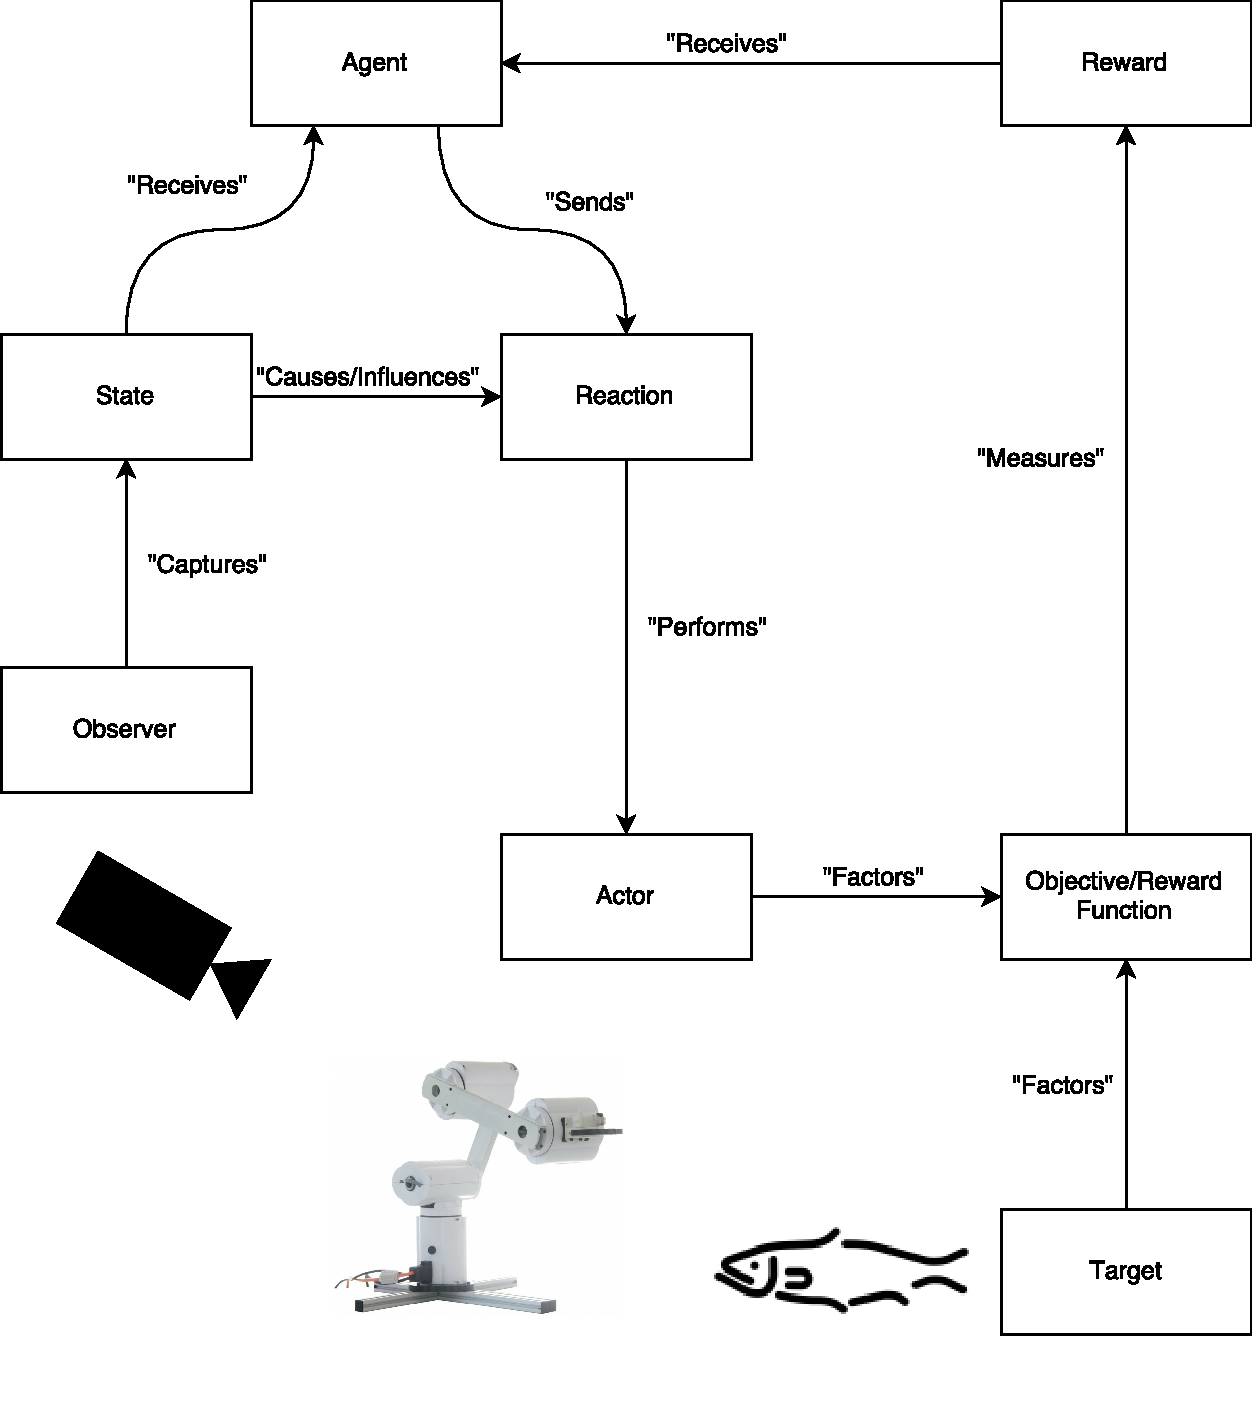
\includegraphics[width=.9\linewidth]{figures/neodroid_classes_verbs.pdf}
\caption{interaction}
\label{fig:interaction}
\end{figure}

Fig.~\ref{fig:interaction} was the result of an effort to build a intuitional mental model for thinking about the environments the agents with be interacting with. Each connection from one entity to another denotes an interactions between these, the direction denotes whether the entity is influenced by or influences the other entity.


\begin{figure}
\centering
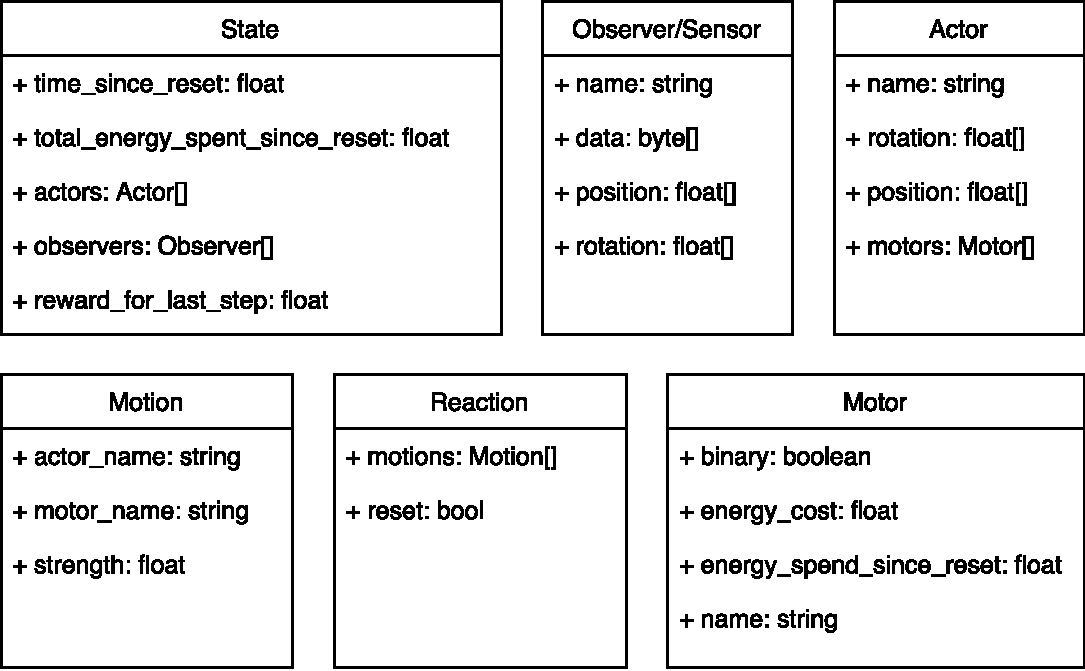
\includegraphics[width=.8\linewidth]{figures/neodroid_classes.pdf}
\caption{classes}
\label{fig:classes}
\end{figure}

Fig.~\ref{fig:classes} is the formalised classes of the earlier interaction activity. Following will be conceptual description of each of the formalised classes.

\subsubsection{Actor}

The concept of the actor model is that is that is encapsulates a number of motors as part of one entity. For example as brushless electric motors on a multirotor aircraft, here the actor is the aircraft and the motors in are the brushless electric motors.

\subsubsection{Agent}

The agent model is an abstraction of some external agent providing reactions to be acted out in the environment. The agent abstraction has the responsibility of providing the interface for external agents into the environment, this include passing messages back and forth through a TCP connection or likewise. 

\subsubsection{Environment State}

The environment state encapsulates all information that should be exposed to external agents into one message. This message is comprised of observers  with their relevant observational data, actors with their positions and rotations in the environments, how much energy has been spent since the last reset, how many frames/time has passed since last reset and lastly a reward given by some objective function.


\subsubsection{Motion}

Motions are abstractions of expenditure of energy and where the energy should be spent. These is simply an address on an actor and a motor with an assigned energy strength, this energy may be positive or negative to indicate for example expansion and contraction of a motor or the torque applied to a motor clock-wise or anti-clock-wise. Its is the absolute magnitude of the strength that counts towards total energy expenditure.
Motions are passed through reaction model as messages produced by the agent, this the way the external agent affect the environment. 

\subsubsection{Motor}

The idea of the motor is very general, is can be unary or binary, here binary refers to the sign of the motion/force being applied to it, if a motor is unary it can only be affected by a positive force.
A motor can apply anything from a spinning motion to a sliding motion, it is easy the realise that both of these can be binary but also unary if chosen. Whereas a rocket motor provide a thrust motion will most likely only be unary.


\subsubsection{Observer}

An observer or its 'sensor' synonym fits quite well for thinking about the abstraction at hand. It is responsible for capturing information in the environment to be passed on the agent. It can for example be used for capturing depth images in the environment or tracking a specific variable in the environment.

\subsubsection{Reaction}

A reaction is the abstraction of a message passed from an external agent to the agent model providing the interface, as a response to the observed state. A reaction includes a boolean variable for resetting the environment and a number of the motion s to be acted out the environment by actor and their motors.

\subsection{Implementation Details}

Serialisation of the data to be transmitted to any external agent, turned out to be quite a bottleneck for running the environment loop at high frame rates. FlatBuffers [https://google.github.io/flatbuffers] was chosen to solve this problem as it is useful for cross compatibility between languages while maintaining low serialisation and deserialisation timings.

\subsection{Objective Functions And Observations}

It should be easy for researchers to include extra terms and individually weight each term to achieve different behaviours of their agents, by the objective function change ever so slightly to reach for minimum in a different function space.

\subsection{Usage Guide}

This section will breifly describe how to use the neodroid interface.

The source code for the python inteface is hosted at \url{https://github.com/sintefneodroid/neo} and the C\# interface at \url{https://github.com/sintefneodroid/droid}.